%package list
\documentclass{article}
\usepackage[top=3cm, bottom=3cm, outer=3cm, inner=3cm]{geometry}
\usepackage{multicol}
\usepackage{graphicx}
\usepackage{url}
%\usepackage{cite}
\usepackage{hyperref}
\usepackage{array}
%\usepackage{multicol}
\newcolumntype{x}[1]{>{\centering\arraybackslash\hspace{0pt}}p{#1}}
\usepackage{natbib}
\usepackage{pdfpages}
\usepackage{multirow}
\usepackage[normalem]{ulem}
\useunder{\uline}{\ul}{}
\usepackage{svg}
\usepackage{xcolor}
\usepackage{listings}
\lstdefinestyle{ascii-tree}{
    literate={├}{|}1 {─}{--}1 {└}{+}1 
  }
\lstset{basicstyle=\ttfamily,
  showstringspaces=false,
  commentstyle=\color{red},
  keywordstyle=\color{blue}
}
%\usepackage{booktabs}
\usepackage{caption}
\usepackage{subcaption}
\usepackage{float}
\usepackage{array}

\newcolumntype{M}[1]{>{\centering\arraybackslash}m{#1}}
\newcolumntype{N}{@{}m{0pt}@{}}


%%%%%%%%%%%%%%%%%%%%%%%%%%%%%%%%%%%%%%%%%%%%%%%%%%%%%%%%%%%%%%%%%%%%%%%%%%%%
%%%%%%%%%%%%%%%%%%%%%%%%%%%%%%%%%%%%%%%%%%%%%%%%%%%%%%%%%%%%%%%%%%%%%%%%%%%%
\newcommand{\itemEmail}{lluquecon@unsa.edu.pe fgarambel@unsa.edu.pe ajrahuacso@unsa.edu.pe wchoquehuancab@unsa.edu.pe}
\newcommand{\itemStudent}{Luis Guillermo Luque Condori, Fernando Miguel Garambel Marín, William Herderson Choquehuanca Berna, Jeans Anthony Ajra Huacso}
\newcommand{\itemCourse}{Laboratorio de P web}
\newcommand{\itemCourseCode}{20233478}
\newcommand{\itemSemester}{III}
\newcommand{\itemUniversity}{Universidad Nacional de San Agustín de Arequipa}
\newcommand{\itemFaculty}{Facultad de Ingeniería de Producción y Servicios}
\newcommand{\itemDepartment}{Departamento Académico de Ingeniería de Sistemas e Informática}
\newcommand{\itemSchool}{Escuela Profesional de Ingeniería de Sistemas}
\newcommand{\itemAcademic}{2024 - A}
\newcommand{\itemInput}{Del 4 de mayo 2024}
\newcommand{\itemOutput}{Al 8 de mayo 2024}
\newcommand{\itemPracticeNumber}{02}
\newcommand{\itemTheme}{Git y GitHub}
%%%%%%%%%%%%%%%%%%%%%%%%%%%%%%%%%%%%%%%%%%%%%%%%%%%%%%%%%%%%%%%%%%%%%%%%%%%%
%%%%%%%%%%%%%%%%%%%%%%%%%%%%%%%%%%%%%%%%%%%%%%%%%%%%%%%%%%%%%%%%%%%%%%%%%%%%

\usepackage[english,spanish]{babel}
\usepackage[utf8]{inputenc}
\AtBeginDocument{\selectlanguage{spanish}}
\renewcommand{\figurename}{Figura}
\renewcommand{\refname}{Referencias}
\renewcommand{\tablename}{Tabla} %esto no funciona cuando se usa babel
\AtBeginDocument{%
	\renewcommand\tablename{Tabla}
}

\usepackage{fancyhdr}
\pagestyle{fancy}
\fancyhf{}
\setlength{\headheight}{30pt}
\renewcommand{\headrulewidth}{1pt}
\renewcommand{\footrulewidth}{1pt}
\fancyhead[L]{\raisebox{-0.2\height}{
\includegraphics[width=3cm]{img/logo_episunsa.png}}}
\fancyhead[C]{\fontsize{7}{7}\selectfont	\itemUniversity \\ \itemFaculty \\ \itemDepartment \\ \itemSchool \\ \textbf{\itemCourse}}
\fancyhead[R]{\raisebox{-0.2\height}{
\includegraphics[width=1.2cm]{img/logo_abet}}}
\fancyfoot[L]{Luis, Fernando, Anthony, William}
\fancyfoot[C]{\itemCourse}
\fancyfoot[R]{Página \thepage}

% para el codigo fuente
\usepackage{listings}
\usepackage{color, colortbl}
\definecolor{dkgreen}{rgb}{0,0.6,0}
\definecolor{gray}{rgb}{0.5,0.5,0.5}
\definecolor{mauve}{rgb}{0.58,0,0.82}
\definecolor{codebackground}{rgb}{0.95, 0.95, 0.92}
\definecolor{tablebackground}{rgb}{0.8, 0, 0}

\lstset{frame=tb,
	language=bash,
	aboveskip=3mm,
	belowskip=3mm,
	showstringspaces=false,
	columns=flexible,
	basicstyle={\small\ttfamily},
	numbers=none,
	numberstyle=\tiny\color{gray},
	keywordstyle=\color{blue},
	commentstyle=\color{dkgreen},
	stringstyle=\color{mauve},
	breaklines=true,
	breakatwhitespace=true,
	tabsize=3,
	backgroundcolor= \color{codebackground},
}

\begin{document}
	
	\vspace*{10px}
	
	\begin{center}	
		\fontsize{17}{17} \textbf{ Informe de Laboratorio \itemPracticeNumber}
	\end{center}
	\centerline{\textbf{\Large Tema: \itemTheme}}
	%\vspace*{0.5cm}	

	\begin{flushright}
		\begin{tabular}{|M{2.5cm}|N|}
			\hline 
			\rowcolor{tablebackground}
			\color{white} \textbf{Nota}  \\
			\hline 
			     \\[30pt]
			\hline 			
		\end{tabular}
	\end{flushright}	

	\begin{table}[H]
		\begin{tabular}{|x{4.7cm}|x{4.8cm}|x{4.8cm}|}
			\hline 
			\rowcolor{tablebackground}
			\color{white} \textbf{Estudiantes} & \color{white}\textbf{Escuela}  & \color{white}\textbf{Asignatura}   \\
			\hline 
			{\itemStudent \par \itemEmail} & \itemSchool & {\itemCourse \par Semestre: \itemSemester \par Código: \itemCourseCode}     \\
			\hline 			
		\end{tabular}
	\end{table}		
	
	\begin{table}[H]
		\begin{tabular}{|x{4.7cm}|x{4.8cm}|x{4.8cm}|}
			\hline 
			\rowcolor{tablebackground}
			\color{white}\textbf{Laboratorio} & \color{white}\textbf{Tema}  & \color{white}\textbf{Duración}   \\
			\hline 
			\itemPracticeNumber & \itemTheme & 04 horas   \\
			\hline 
		\end{tabular}
	\end{table}
	
	\begin{table}[H]
		\begin{tabular}{|x{4.7cm}|x{4.8cm}|x{4.8cm}|}
			\hline 
			\rowcolor{tablebackground}
			\color{white}\textbf{Semestre académico} & \color{white}\textbf{Fecha de inicio}  & \color{white}\textbf{Fecha de entrega}   \\
			\hline 
			\itemAcademic & \itemInput &  \itemOutput  \\
			\hline 
		\end{tabular}
	\end{table}
	
	\section{Actividades}
	\begin{itemize}		
		\item Cree una cuenta de usuario en github
		\item Configure su cuenta de estudiante (https://education.github.com/pack).
	\end{itemize}
\section{Ejercicios Propuestos}
	\begin{itemize}		
		\item Forme grupos de 3 a 5 personas
		\item Un integrante del grupo deberá crear el proyecto principal, con el nombre de su grupo, con la plantilla base
		\item Comparta el proyecto con sus compañeros de grupo y asigne uno o dos  métodos distintos a cada integrante del grupo.
		\item Los integrantes del grupo deberán hacer clone, push y pull según corresponda, de modo que el repositorio contenga la solución final.
		\item Reportar al profesor que logró culminar la tarea. La tarea debe ser compartida con el profesor (CarloCorralesD) y entregada usando el mismo url que se usó para clonar el repositorio.
	\end{itemize}

	\section{Equipos, materiales y temas utilizados}
	\begin{itemize}
		\item Sistema operativo de 64 bits, procesador basado en x64.
		\item Latex. 
		\item git version 2.41.0.windows.1
		\item Cuenta en GitHub con el correo institucional.
	\end{itemize}
	\section{URL Github, Video}
	\begin{itemize}
		\item URL del Repositorio GitHub para clonar o recuperar.
		\item \url{https://github.com/FernandoGarambelM/Calculadora-pw2-.git}
		\item URL para el video flipgrid.
		\item \url{https://flip.com/s/NoTBBoy8MByz}	
	\end{itemize}
	\clearpage
	\section{Capturas de pantalla de la cuenta y la version}
		\subsection{Captura de Fernando Miguel Garambel Marín}
	\begin{itemize}
		\item Version
	\end{itemize}
	\begin{figure}[H]
		\centering
		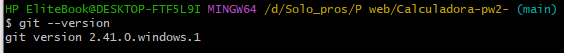
\includegraphics[width=1.0\textwidth,keepaspectratio]{img/FernandoVersion.PNG}
		%\includesvg{img/automata.svg}
		%\label{img:mot2}
		%\caption{Product backlog.}
	\end{figure}
	\begin{itemize}
		\item Cuenta creada
	\end{itemize}
	\begin{figure}[H]
		\centering
		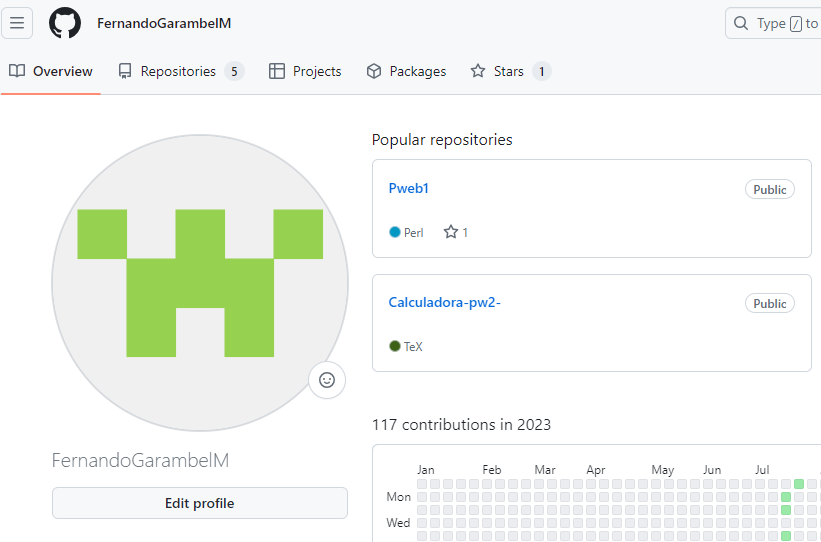
\includegraphics[width=1.0\textwidth,keepaspectratio]{img/FernandoCuenta.PNG}
		%\includesvg{img/automata.svg}
		%\label{img:mot2}
		%\caption{Product backlog.}
	\end{figure}
	\clearpage
	\subsection{Captura de Jeans Anthony Ajra Huacso}
	\begin{itemize}
		\item Version
	\end{itemize}
	\begin{figure}[H]
		\centering
		
\includegraphics[width=1.0\textwidth,keepaspectratio]{img/AnthonyVersion.jpg}
		%\includesvg{img/automata.svg}
		%\label{img:mot2}
		%\caption{Product backlog.}
	\end{figure}
	\begin{itemize}
		\item Cuenta creada
	\end{itemize}
	\begin{figure}[H]
		\centering
		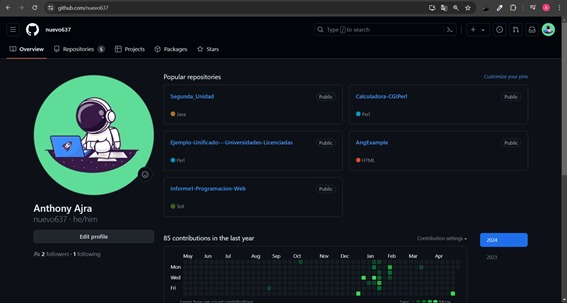
\includegraphics[width=1.0\textwidth,keepaspectratio]{img/AnthonyCuenta.jpg}
		%\includesvg{img/automata.svg}
		%\label{img:mot2}
		%\caption{Product backlog.}
	\end{figure}
	\clearpage
	\subsection{Captura de Luis Guillermo Luque Condori}
	\begin{itemize}
		\item Version
	\end{itemize}
	\begin{figure}[H]
		\centering
		
\includegraphics[width=1.0\textwidth,keepaspectratio]{img/LuisVersion.jpg}
		%\includesvg{img/automata.svg}
		%\label{img:mot2}
		%\caption{Product backlog.}
	\end{figure}
	\begin{itemize}
		\item Cuenta creada
	\end{itemize}
	\begin{figure}[H]
		\centering
		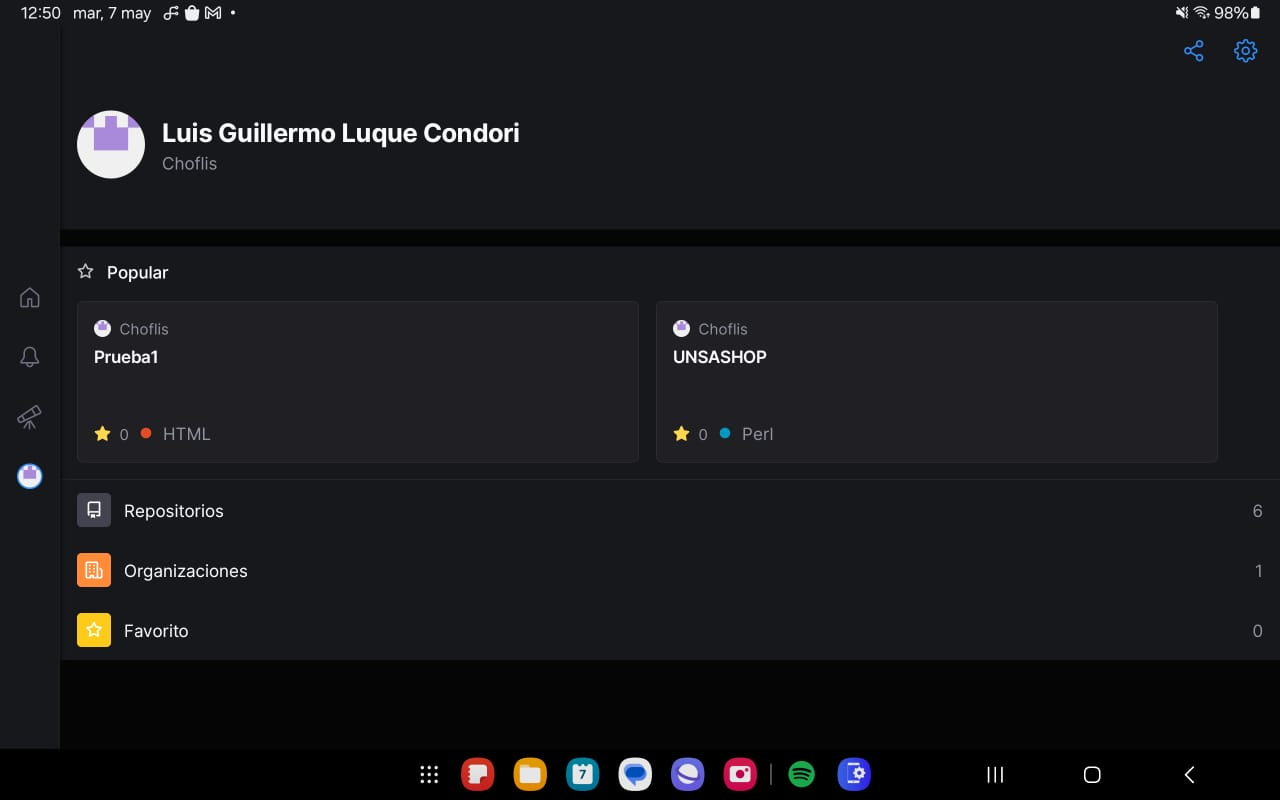
\includegraphics[width=1.0\textwidth,keepaspectratio]{img/LuisCuenta.jpg}
		%\includesvg{img/automata.svg}
		%\label{img:mot2}
		%\caption{Product backlog.}
	\end{figure}
	\clearpage
	\subsection{Captura de William Herderson Choquehuanca Berna}
	\begin{itemize}
		\item Version
	\end{itemize}
	\begin{figure}[H]
		\centering
		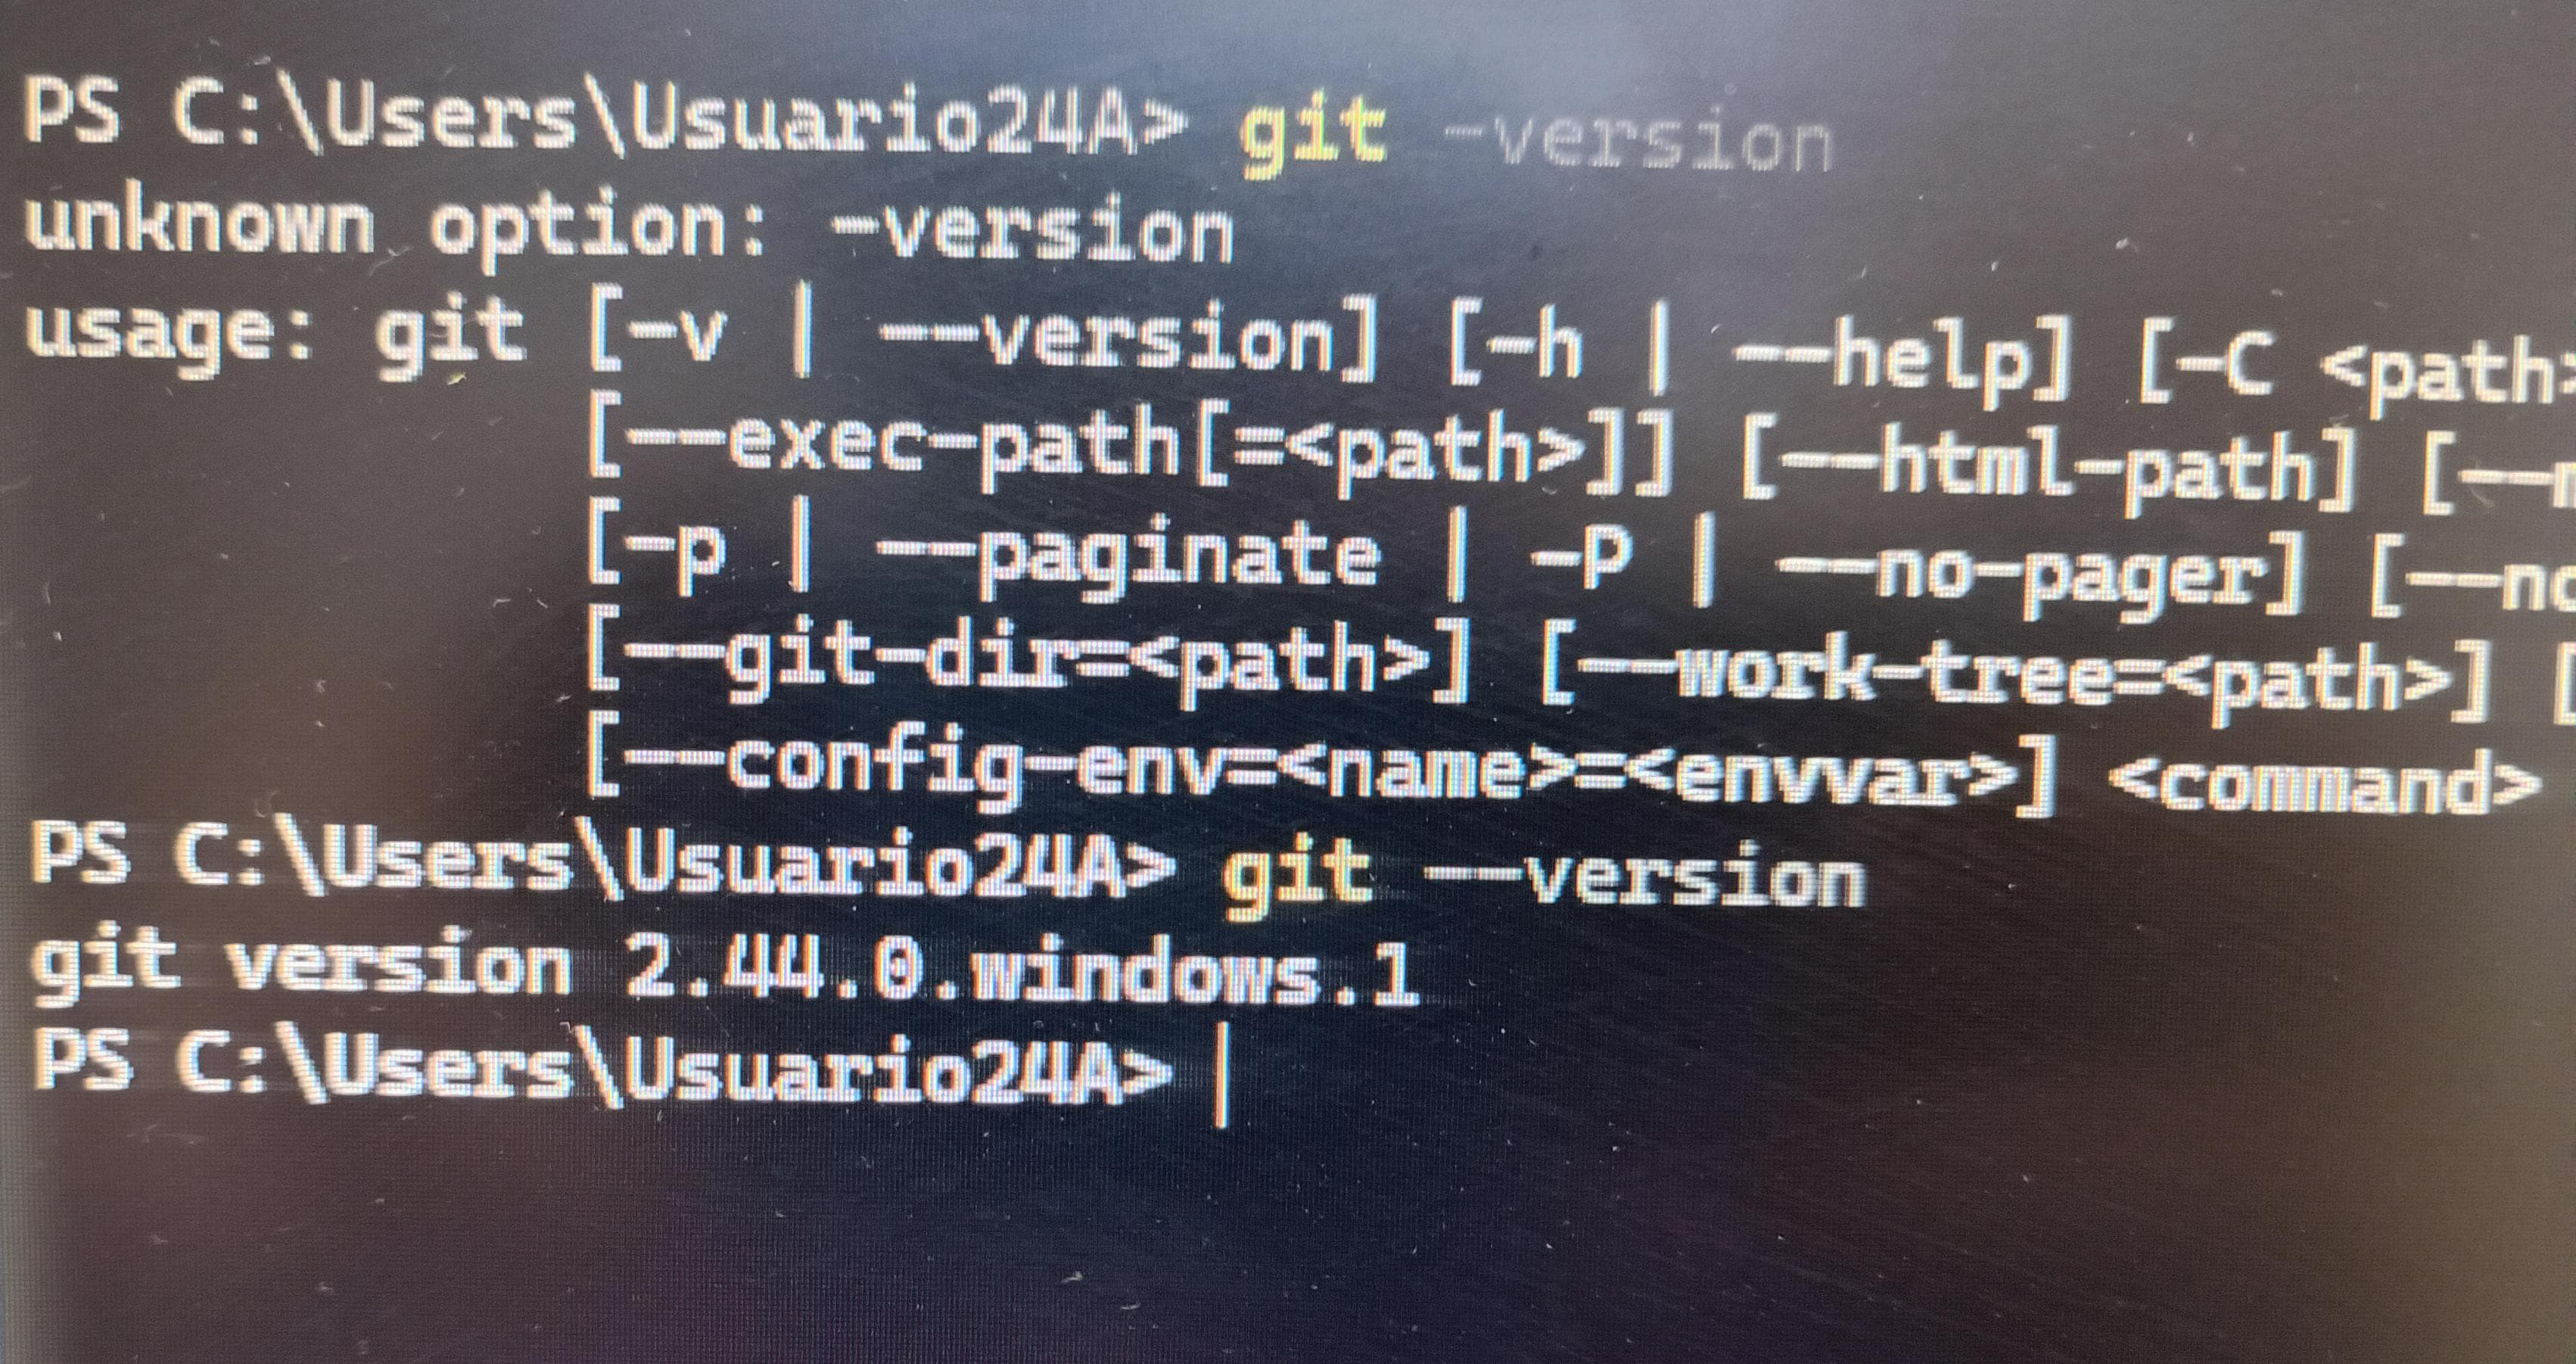
\includegraphics[width=1.0\textwidth,keepaspectratio]{img/WilliamVersion.jpg}
		%\includesvg{img/automata.svg}
		%\label{img:mot2}
		%\caption{Product backlog.}
	\end{figure}
	\begin{itemize}
		\item Cuenta creada
	\end{itemize}
	\begin{figure}[H]
		\centering
		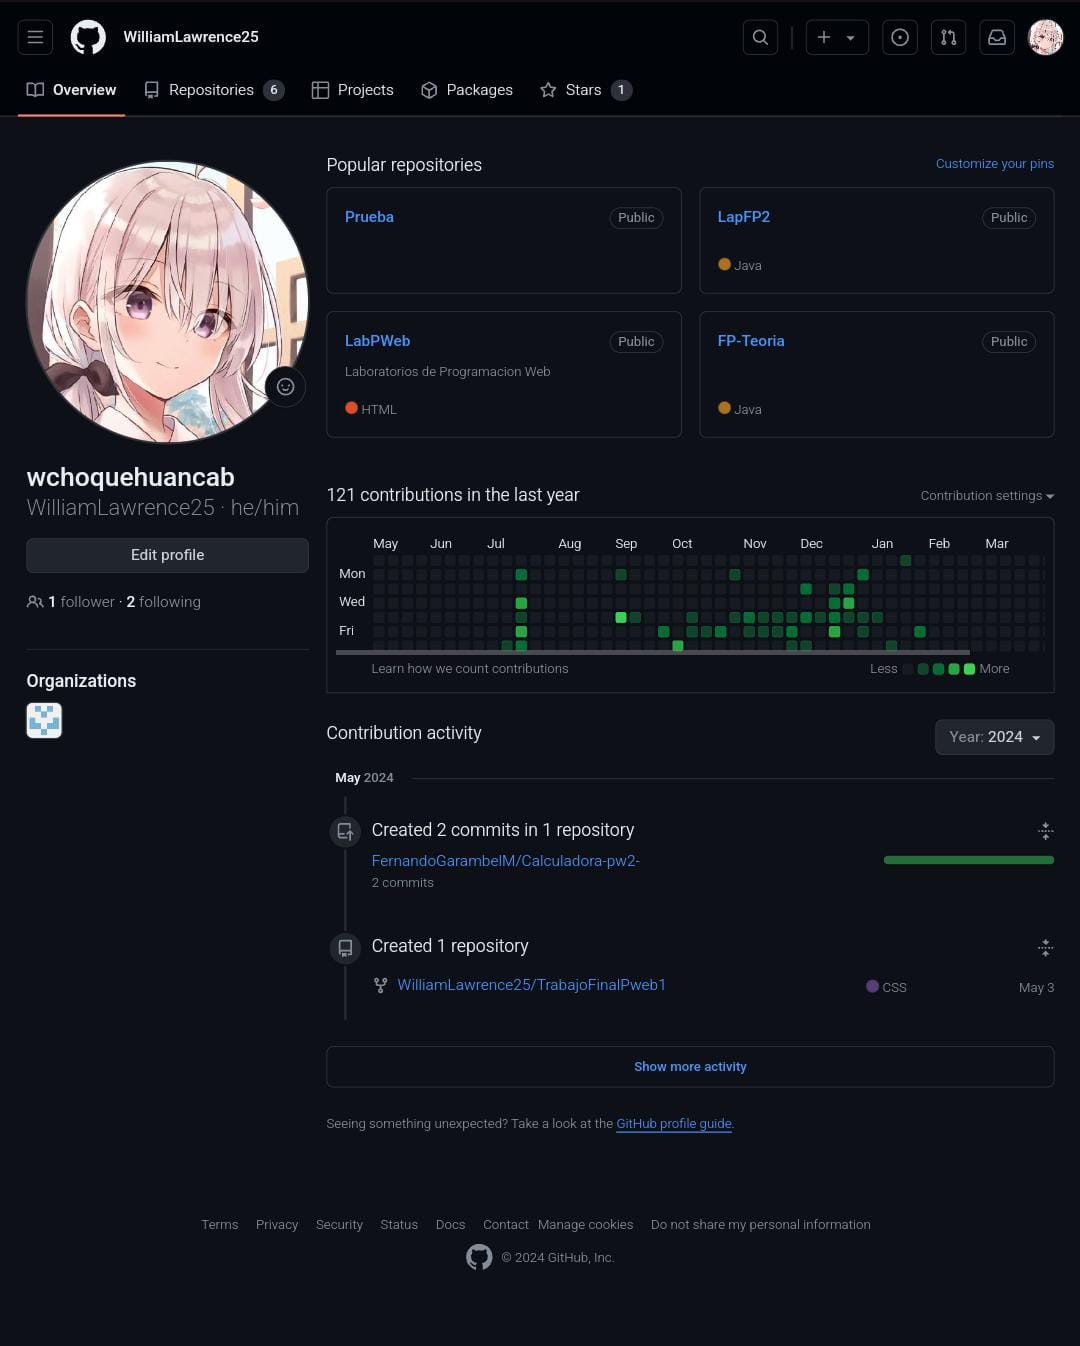
\includegraphics[width=1.0\textwidth,keepaspectratio]{img/WilliamCuenta.jpg}
		%\includesvg{img/automata.svg}
		%\label{img:mot2}
		%\caption{Product backlog.}
	\end{figure}
	\clearpage
\section{Calculadora en Java}
	\subsection{Clase Calculator}
	\lstinputlisting[language=Java, caption={Código de Calculator},numbers=left,]{src/Calculator.java}
	\begin{itemize}
		\item  A continuación se explicaran los métodos utilizados en Calculator.
	\end{itemize}
	\subsection{Método add}
	\begin{lstlisting}[language=bash,caption={Código del método add}][H]
		int add(int a, int b){
        		int resultado = a + b;
        		return resultado;
    		}	
	\end{lstlisting}
	\begin{itemize}
		\item  Para utilizar este método se creó el método sumar que es el que interactua con el usuario
	\end{itemize}
	\begin{lstlisting}[language=bash,caption={Código del método sumar}][H]
	public void sumar(){
        System.out.println("Ingrese los dos numeros a sumar: ");
        System.out.print("Numero 1: ");
        int a = sc.nextInt();
        System.out.print("Numero 2: ");
        int b = sc.nextInt();
        int resultado = add(a, b);
        System.out.println("El resultado de la suma es: " + resultado + "\n");
    }	
	\end{lstlisting}
	\subsection{Método sub}
	\begin{lstlisting}[language=bash,caption={Código del método sub}][H]
		int sub(int a, int b){
        int resultado = a - b;
        return resultado; 
    }	
	\end{lstlisting}
	\begin{itemize}
		\item  Para utilizar este método se creó el método restar que es el que interactua con el usuario
	\end{itemize}
	\begin{lstlisting}[language=bash,caption={Código del método restar}][H]
		public void restar(){
			System.out.println("Ingrese los dos numeros a restar: ");
			System.out.print("Numero 1: ");
			int a = sc.nextInt();
			System.out.print("Numero 2: ");
			int b = sc.nextInt();
			int resultado = sub(a, b);
			System.out.println("El resultado de la resta es: " + resultado + "\n");
		}	
	\end{lstlisting}
	\subsection{Método mul}
	\begin{lstlisting}[language=bash,caption={Código del método mul}][H]
		int mul(int a, int b){ 
        int resultado = a * b;
        return resultado; 
    }	
	\end{lstlisting}
	\begin{itemize}
		\item  Para utilizar este método se creó el método multiplicar que es el que interactua con el usuario
	\end{itemize}
	\begin{lstlisting}[language=bash,caption={Código del método multiplicar}][H]
		public void multiplicar(){
        System.out.println("Ingrese los numeros: ");
        int a = sc.nextInt();
        int b = sc.nextInt();
        int resultado = mul(a, b);
        System.out.println("El resultado de la operacion es: " + resultado);
    }
	\end{lstlisting}
	\subsection{Método dividirNumeros}
	\begin{lstlisting}[language=bash,caption={Código del método dividirNumeros}][H]
		public void dividirNumeros() {
        System.out.println("Ingrese los numeros: ");
        double dividendo = sc.nextDouble();
        double divisor = sc.nextDouble();

        if (divisor == 0) {
            System.out.println("Error: No se puede dividir por cero.");
        }

        double respuesta = dividendo / divisor;
        System.out.println("El resultado es: " + respuesta);
 
    }
	\end{lstlisting}
	\subsection{Método mod}
	\begin{lstlisting}[language=bash,caption={Código del método mod}][H]
		int mod(int a, int b){
        int resultado = a % b;
        return resultado; 
    }
	\end{lstlisting}
	\begin{itemize}
		\item  Para utilizar este método se creó el método modulo que es el que interactua con el usuario
	\end{itemize}
	\begin{lstlisting}[language=bash,caption={Código del método modulo}][H]
		public void modulo(){
        System.out.println("Ingrese los numeros: ");
        int a = sc.nextInt();
        int b = sc.nextInt();
        System.out.println("El resultado de la operacion es: " + mod(a, b));
    }
	\end{lstlisting}
	\subsection{Main}
	\lstinputlisting[language=Java, caption={Código Main},numbers=left,]{src/Main.java}
	\begin{itemize}
		\item Este método es el que usa todos los métodos de calculator y hace la calculadora al final.
	\end{itemize}
	
	\clearpage
\section{Referencias}
\begin{itemize}			
	\item \url{https://www.w3schools.com/java/default.asp}
\end{itemize}	
	
%\clearpage
%\bibliographystyle{apalike}
%\bibliographystyle{IEEEtranN}
%\bibliography{bibliography}
			
\end{document}